\section{Travelling Wave Analysis}

This will be the beefy section that details the travelling wave analysis.
Some things to include here
\begin{itemize}
  \item show that the 2d-region problem can be reduced to a 1d-problem with appropriatly homogenous initial conditions in one of the dimensions (x2?)
   \item Show the typical solution of the travelling wave
   \item Show computations for the wave speed
   \item (if I get this working) show the results of the wavespeed as a function of $\mu, \delta, \nu, \gamma, \kappa$ in a panel plot sort of thing.
\end{itemize}


\subsection{Problem Specifics}

This will quickly list the main differences between the simulations that will be done here compared to the typical simulations of the previous section.
Mainly just list the new initial conditions etc.

\subsection{Reduce Spatial Dimension}

%!% THERE IS ONE HUGE ISSUE WITH THIS SECTION, THE X-Y AXIS THING NEEDS TO BE SWAPED. SO THAT THE Y AXIS IS THE ONE BEING REMOVED AND ONLY THE X-Z AXIS IS NEEDED FOR VISUALIZATION.... MAKE SURE THE MATH CHECKS OUT WITH THIS CHANGE WHEN IT IS MADE.

  The system (\ref{equ:model_system} - \ref{equ:model_functions}) can be reduced to a $1D$ problem. 
  
  %!% ADD HERE THE BASICS FOR THE TRAVELLING WAVE SCENARIO (HOMOGENOUS IC ON REGION BOUNDARY)
  
  Since the initial conditions are homogenous with respect to x, the x axis can be ignored and only the y-z axis is needed for visualization. Looking at Figure \ref{fig:visual}, the homoginity is clear.
   
  \begin{figure}[h!bt]
    \begin{center}
      \begin{tabular}{c c}
%        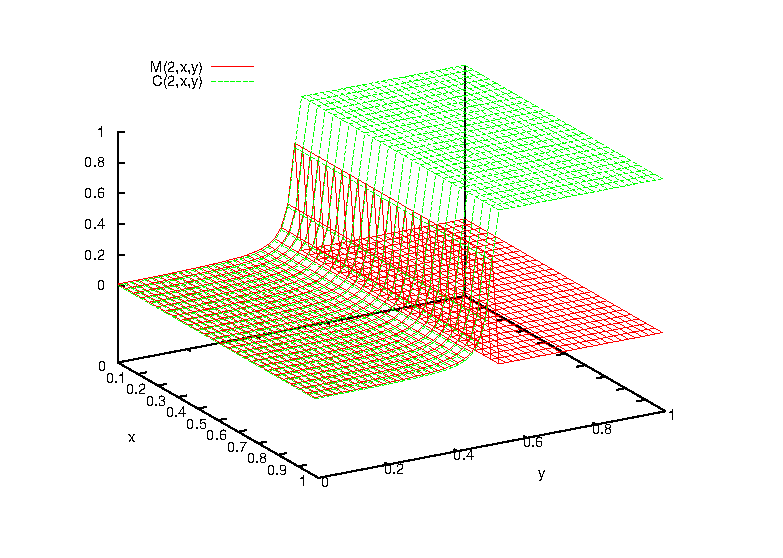
\includegraphics[scale=0.5]{view_3D.eps} &
%        \includegraphics[scale=0.5]{view_psuedo2D.eps} \\
        (a) & (b) \\
      \end{tabular}
      \caption{Graph of (a) 3D view of $M(t,x,y)$ and $C(t,x,y)$, (b) Side profile view of $M(t,x,y)$ and $C(t,x,y)$ at $t=2$.} 
      \label{fig:visual}
    \end{center}
  \end{figure}
   
    This can be shown quantitatily by comparing the maximum and minimum values of M and C with respect to the x-axis (Figure \ref{fig:maxMin}). 
  \begin{figure}[h!bt]
    \begin{center}
%        \includegraphics[scale=0.8]{maxMin_MC.eps}
      \caption{Graph of difference between max and min of M and difference between max and min of C.}
      \label{fig:maxMin}
    \end{center}
  \end{figure}

  The difference between the max and min remains constant with respect to time (Table \ref{tab:overTime}), this was calculated by,
  \begin{equation}
    \begin{aligned}
      \delta_M(t) &= \frac{1}{256}\sum_{i = 1}^n \left( \sup_{j \in (1,m)} M(x_i,y_j) - \inf_{k \in (1,m)} M(x_i,y_k) \right) \\
      \delta_C(t) &= \frac{1}{256}\sum_{i = 1}^n \left( \sup_{j \in (1,m)} C(x_i,y_j) - \inf_{k \in (1,m)} C(x_i,y_k) \right)   
    \end{aligned}
  \end{equation}
  
   \begin{table}
    \begin{center}
      \begin{tabular}{| c | c | c |} 
        \hline
        t & $\delta_M$ & $\delta_C$ \\
        \hline
        0.0 & 0.0 & 0.0037109375 \\
        0.5 &1.71577851563e-06 & 0.00371116503633\\
        1.0 &7.62408671875e-06 & 0.00371156747773\\
        1.5 &9.04633828125e-06 & 0.00371216829336\\
        2.0 &7.648728125e-06 & 0.00371311224609\\
        2.5 &2.58707890625e-06 & 0.00371457725742\\
        3.0 &0.00162623974609 & 0.00240237613672\\
        3.5 &5.35270417969e-05 & 7.24265101562e-05\\
        4.5 &1.07250539062e-05 & 2.12679726563e-05 \\
        5.0 &1.09254414063e-06 & 9.720734375e-06\\
        \hline
      \end{tabular}
      \caption{A table of values for $\delta_M(t)$ and $\delta_C(t)$}
      \label{tab:overTime}
    \end{center}
  \end{table}
   
   So by taking the average of the points along the $x$-axis we can get a 2D plot as seen in Figure \ref{fig:true2D}. 
   
 
  \begin{figure}[h!bt]
    \begin{center}
%        \includegraphics[scale=0.8]{view_2D.eps}
      \caption{Graph of M(2,y) and C(2,y), now reduced to a 2D plot.}
      \label{fig:true2D}
    \end{center}
  \end{figure}




\subsection{Typical Travelling Wave Simulation}

The system
\begin{align}
    M_t &= \nabla_x \left( D(M) \nabla_x M \right) + f(C) M \\
    C_t &= - g(C) M 
\end{align}
where
\begin{align}
    D(M) &= \delta \frac{M^\alpha}{(1 - M)^\beta} \\
    f(C) &= g(C) - \nu  \\
    g(C) &= \frac{\gamma C}{\kappa +C}
\end{align}
is solved on a rectangular region with length $L$ and width $\lambda L$ with the following parameter values,
\begin{equation}
\begin{aligned}
    \alpha &= 4 \\
    \beta &= 4 \\
    \nu &= 0.1 
\end{aligned}
\qquad
\begin{aligned}
    \delta &= 10^{-8} \\
    \kappa &= 0.01\\
    \gamma &= 0.81
\end{aligned}
\end{equation}
and with initial conditions 
\begin{equation}
\begin{aligned}
    C &= 1 \\
    M &= \begin{cases} -(\frac{h}{d^4})x^4 + h & \text{if } x < 0.04 \\ 0 & \text{otherwise }\end{cases} \\
\end{aligned}
\end{equation}  
where $h = 0.1, d=\frac{5}{128}$ , representing the height and depth of the inoculation site.

Using simulation code version $139e63e$ the possibilty of a travelling wave solution existing was examined. The following results were found using a finite difference method to solve $M$ and trapizedral rule to solve $C$ with $\Delta x = \frac{1}{1024}$ and $\Delta t = 10^-2$.



\begin{figure}[h!tb]
\begin{center}
  \begin{tabular}{c c}
      \includegraphics[scale=0.55]{solution_t0.eps} &
      \includegraphics[scale=0.55]{solution_t13.eps} \\
      (a) & (b) \\
      \includegraphics[scale=0.55]{solution_t26.eps} &
      \includegraphics[scale=0.55]{solution_t40.eps} \\
      (c) & (d) 
  \end{tabular}
  \caption{Solutions of $M(x,t)$ and $C(x,t)$ at (a) t = 0, (b) t = 26, (c) = 52, (d) = 80. }
  \label{fig:solution}
\end{center}
\end{figure}

The solution to the above system can be seen in Figure \ref{fig:solution}. This solution seems to have characteristics of a travelling wave solution. This is because after $t=60$, we can write the solution $M(x,t)$ as $M(x-ct)$, where $c$ is the wavespeed of the solution. We can numerically approximate the value for $c$ by looking at how fast the peak of the wave travels, Figure \ref{fig:waveSpeed} shows that this value is $c \approx c^n = 5.3533 \times 10^{-3}$. Now we can show that the solutions can be written as $M(x-ct)$ by shifting solutions of $M(x,t)$ by $\pm n_i c$, with $n_i \in \mathbb{Z}$, as seen in Figure \ref{fig:travShape}.

\begin{figure}[h!tb]
\begin{center}
    \includegraphics[scale=0.85]{wavespeed.eps}
    \caption{Max $M$ value as a function of $t$. The green line is an approximation for the wavespeed, $c = 5.3533 * 10^{-3}$.}
    \label{fig:waveSpeed} 
\end{center}
\end{figure}

This is just a bunch of filler text to see if things will work.

\begin{figure}[h!tb]
\begin{center}
    \includegraphics[scale=0.85]{travShape.eps}
    \caption{Solutions of $M(x+ct)$ at time $t_i = 0 \ldots 10$ each horizontally translated by $-n_i c t_d$, where $n_i = 0 \ldots 10$,  $c = 5.3533 \times 10^{-3}$, and $t_d = t_i - t_{i-1} $}
    \label{fig:travShape}
\end{center}
\end{figure}


\subsection{Wave Speed}

This will be a quick section that shows the change of wave speed as a function of the different parameters.

A few notes for the figure below, Figure \ref{fig:paramwavespeed}. This should be a GNUplot multiplot. With the four different plots ordered in a 4x1 column. If I try having the traveling wave existance thing implemented, then have a greyed out box for the sections without travelling waves.

\begin{figure}
  \centering
  %\includegraphics[scale=0.85]{wavespeedparam.eps}
  \caption{The value of $c$ as single parameters are changed. (a) $\delta$, (b) $\kappa$, (c) $\nu$, (d) $\gamma$. }
  \label{fig:paramwavespeed}
\end{figure}


